\section{Experimental Results}\label{sec:experiments}

\subsection{Setup}\label{sec:setup}

We evaluate on all seven ICCAD 2024 CAD Contest Problem~B benchmarks~\cite{yang2024contest,fang2024overview}: three released and four hidden cases spanning millions of instances and widely different weight profiles. All scores are from the official preliminary evaluator on the final solution file; every solution passed its legality check and the contest sanity and placement checkers. The flow is C++ with OpenMP on the strengthened open-source front end~\cite{baselineRepo} of Section~\ref{sec:background}; refinement deltas are measured against that strengthened base, not the stock public flow.

All results use one unified configuration: a single recipe, zero per-case hyperparameters. The recipe was fixed via no-regression sweeps over the same seven cases, so like all published results on this benchmark it is selected in-sample. Unlike them, no knob differs between cases, and it beat every per-case-tuned configuration this flow had produced. We will release all seven solution files for independent checking. Experiments ran on a dual Intel Xeon E5-2630~v4 server (2.2\,GHz, 40 logical cores, 94\,GB RAM) with 8 threads. Operators run to convergence fixpoints, so results are reproducible: six of seven cases are byte-identical across all three repeats. On Hidden~4 one accept's gain sits at floating-point noise and flips between repeats, moving the final score by $2{\times}10^{-4}$\,\% (std/mean).

\subsection{Main Results}\label{sec:mainresults}

Table~\ref{tab:main} compares against every evaluator-comparable published result: the top-3 per-case contest costs, the winner's method LBR (a two-page late-breaking result~\cite{li2025lbr}, self-reported average ratio 0.988 vs.\ first place), and the DATE~2026 flow~\cite{chen2026agile}, self-reported $0.2\%$ better than LBR on average. Ours alone beats the top-3 best on every case and wins all seven head to head: vs.\ LBR by $2.0\%$ on Case~2 and $20.9\%$ on Hidden~2, vs.\ DATE'26 by $4.3\%$ and $12.3\%$. The composite does not hinge on one case: the geometric mean is 0.949, and excluding Hidden~2 still yields 0.986, ahead of both methods recomputed on the same six cases (LBR 0.997, DATE'26 0.999). Hidden~2's margin is mechanistic: on this power-dominated case, proxy-priced flows leave $2{\times}2\mathrm{b}{\to}4\mathrm{b}$ merges unexploited that exact pricing captures safely. TIMBER~\cite{dassarma2026timber} also reports on these cases, but under its own min--max normalization and a baseline re-run whose bin-violation counts differ from the official contest standings; its scores cannot be placed in this table. Its strengths are runtime and memory rather than the contest cost metric.

\begin{table*}[t]
\centering
\caption{Official evaluator scores on all seven Problem~B cases (lower is better). Top-3 costs re-evaluated in~\cite{chen2026agile}; LBR scores as published (four significant digits)~\cite{li2025lbr}. Ratios and composites (average per-case ratio) use the same top-3-best baseline. Baselines in print differ slightly (Case~2 first place: 748{,}000 in~\cite{li2025lbr} vs.\ 744{,}231 in~\cite{chen2026agile}); we use the stricter, so our margins are conservative.}
\label{tab:main}
\small
\begin{tabular}{@{}lrrrrrr@{}}
\toprule
Case & Top-3 best & LBR~\cite{li2025lbr} & DATE'26~\cite{chen2026agile} & Ours & $\Delta$ vs top-3 & T (s) \\
\midrule
Case 1   & 739{,}235{,}861 & 738{,}800{,}000 & 736{,}602{,}486 & \textbf{734{,}766{,}838} & $-0.60\%$ & 199 \\
Case 2   & 744{,}231       & 738{,}400       & 756{,}559       & \textbf{723{,}780}       & $-2.75\%$ & 1{,}216 \\
Case 3   & 727{,}971{,}140 & 728{,}800{,}000 & 727{,}757{,}372 & \textbf{726{,}236{,}872} & $-0.24\%$ & 2{,}582 \\
Hidden 1 & 31{,}507{,}917  & 31{,}270{,}000  & 30{,}946{,}401  & \textbf{30{,}199{,}301}  & $-4.15\%$ & 203 \\
Hidden 2 & 13{,}408{,}414  & 12{,}760{,}000  & 11{,}510{,}067  & \textbf{10{,}097{,}053}  & $-24.70\%$ & 2{,}202 \\
Hidden 3 & 55{,}941{,}500  & 55{,}920{,}000  & 55{,}973{,}041  & \textbf{55{,}789{,}826}  & $-0.27\%$ & 1{,}787 \\
Hidden 4 & 728{,}497{,}353 & 726{,}900{,}000 & 727{,}798{,}594 & \textbf{726{,}154{,}906} & $-0.32\%$ & 2{,}619 \\
\midrule
Composite & 1.000 & 0.991 & 0.979 & \textbf{0.953} & & \\
\bottomrule
\end{tabular}
\end{table*}

\subsection{Ablation}\label{sec:ablation}

Table~\ref{tab:ablation} enables the operators cumulatively on the three most cost-sensitive cases. The base row is the strengthened proxy-priced front end of Section~\ref{sec:background} with refinement disabled, so deltas attribute to refinement only. Attribution tracks per-case cost structure. Exact batch re-pairing is the largest lever everywhere ($-0.9\%$ to $-8.6\%$). Move-space repair (an audit finding, not an algorithmic contribution) and structural rebanking pay where residual cost sits in banking structure (Case~2, Hidden~2); rebanking alone gives $-1.4\%$ and $-2.5\%$ respectively. Density pricing only acts where bins overfill: it moves Hidden~1 by $-0.4\%$ and is a verified no-op on Case~2 and Hidden~2, whose bin counts are already legal. No stage regresses any of the three cases.

A controlled counterfactual isolates pricing: we rerun the full flow unchanged except that the inherited one-hop proxy quotes each rebanking accept; candidates, staging, and operators are identical. Every case degrades: $+0.15\%$ on Case~2, $+0.90\%$ on Hidden~1, $+0.41\%$ on Hidden~2. Exact pricing therefore wins even inside an identical architecture. The staged monotone commit structure separately contains the damage that historically compounded under in-flow proxy merging (Sec.~\ref{sec:background}); those cascades required losing both safeguards.

\begin{table}[t]
\centering
\caption{Cumulative ablation, official evaluator score (lower is better).}
\label{tab:ablation}
\footnotesize
\begin{tabular}{@{}lrrr@{}}
\toprule
Configuration & Case 2 & Hidden 1 & Hidden 2 \\
\midrule
Front end (no refinement)       & 761{,}159 & 30{,}615{,}486 & 11{,}614{,}120 \\
$+$ exact batch re-pairing      & 740{,}251 & 30{,}336{,}791 & 10{,}619{,}091 \\
$+$ move-space repair           & 733{,}903 & 30{,}335{,}019 & 10{,}356{,}851 \\
$+$ structural rebanking        & 723{,}780 & 30{,}327{,}025 & 10{,}097{,}053 \\
$+$ density-term pricing        & 723{,}780 & 30{,}199{,}301 & 10{,}097{,}053 \\
\bottomrule
\end{tabular}
\end{table}

\subsection{Anytime Behavior}\label{sec:anytime}

Figure~\ref{fig:anytime} plots official evaluator score against refinement wall-clock for the two cases with the most headroom; each point is one evaluator run at a stage boundary, and the descent is monotone across all 63 checkpoints on all seven cases.

\begin{figure}[t]
\centering
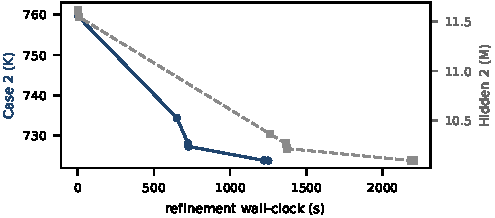
\includegraphics[width=\linewidth]{figs/anytime.pdf}
\caption{Official evaluator score versus refinement wall-clock. Case~2 (left axis, solid) and Hidden~2 (right axis, dashed).}
\label{fig:anytime}
\end{figure}

\subsection{Runtime}\label{sec:runtime}

Table~\ref{tab:main} lists per-case wall times; the full suite takes about three hours on one server. Cases that converge fast finish in under four minutes, and TNS-bound cases spend where descent continues. Bit re-pairing dominates (66--96\% of refinement time); rebanking takes 4--108\,s per case; density repair finishes in under 0.1\,s everywhere and is a no-op on the three cases without overfilled bins.

The runtime--quality trade can be quoted at any budget: a 1--2.5 minute refinement cap (median 120\,s wall) yields composite 0.966, a 3--8 minute class 0.958, and full convergence 0.953. Every point beats the best published composite (0.979). At LBR's runtime class ours is already 2.5 points ahead; the two-minute tier meets contest-style budgets by construction.

The base flow completes in 21--36\,s, comparable to the contest entries; the extra budget buys millions of exactly-priced moves that faster flows never attempt (on Hidden~2, screening prices about 4{,}000 structural candidates per second at 8 threads, and one exact trial-apply costs $\sim$12\,ms). For reference, DATE~2026 reaches 0.979 in ${\sim}3$\,s per case (2.5\,GHz i7~\cite{chen2026agile}), LBR 0.991 in up to 77\,s (3\,GHz EPYC~\cite{li2025lbr}), and ours 0.953 in minutes on an older 2.2\,GHz server.
